\usetikzlibrary{arrows.meta,calc,matrix,shapes}
\providecommand{\computer}{%
    
\includegraphics[width=1cm]{../common/Noun_project_216.pdf}
}
\providecommand{\switch}{%
    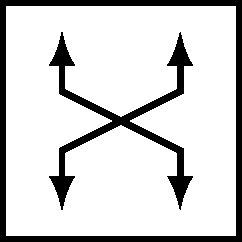
\includegraphics[width=0.9cm]{../common/fig-switch.pdf}
}
\providecommand{\router}{%
    
\includegraphics[width=0.9cm]{../common/fig-router.pdf}
}

\begin{frame}{basic flooding}
    \begin{itemize}
    \item idea: broadcast message to whole network
    \item where message comes from = way to send back
    \vspace{.5cm}
    \item used this idea in MAC learning
    \end{itemize}
\end{frame}

\begin{frame}{flooding one entry}
\begin{tikzpicture}
\tikzset{
    computer/.style={inner sep=0mm,outer sep=0mm,execute at begin node={\computer}},
    switch/.style={inner sep=0mm,outer sep=0mm,execute at begin node={\switch}},
    connect/.style={draw,very thick,Latex-Latex},
    connect big/.style={draw,ultra thick,Latex-Latex},
    port/.style={pos=0.95,fill=white,circle,draw,inner sep=0mm},
    port beginning/.style={pos=0.05,fill=white,circle,draw,inner sep=0mm},
    route table/.style={
        matrix of nodes,ampersand replacement=\&,
        column 1/.style={nodes={draw,thick,text width=2.5cm,font=\tiny\tt,text depth=0mm,minimum height=0.5cm,inner sep=1mm}},
        column 2/.style={nodes={draw,thick,text width=.5cm,font=\small\tt,text depth=0mm,minimum height=0.5cm,inner sep=1mm}},
        row 1/.style={nodes={draw=none,font=\small}},
    },
    mac label/.style={
        draw,fill=white,inner sep=1mm,font=\tiny\tt,
    },
}
\foreach \x/\d/\mc/\dir in {15/8cm/AA/north,45/3cm/BB/north,90/2cm/CC/north,135/3cm/DD/north,180/4cm/EE/north,300/4cm/FF/south} {
    \node[computer,label={[mac label,]\dir:00:11:22:33:44:\small\mc}] (c-\x) at (\x:\d) {};
}
\node[switch] (s1) at (4,-0.5) {};
\matrix[route table,anchor=north west,
    row 3/.style={nodes={visible on=<2->,alt=<2>{fill=red!10}}},
] (s1 table) at ([xshift=1cm,yshift=.5cm]s1.north east) {
dst MAC addr \& port \\
\ldots \& \ldots \\
00:11:22:33:44:\small AA \& 1 \\
};
\draw[dotted,thick] (s1.north east) -- (s1 table-2-1.north west);
\draw[dotted,thick] (s1.south east) -- (s1 table-2-1.south west);
\node[switch] (s2) at (-1,0.5) {};
\matrix[route table,
    row 3/.style={nodes={visible on=<3->}},
,anchor=north east] (s2 table) at ([xshift=3cm]s2.south west) {
dst MAC addr \& port \\
\ldots \& \ldots \\
00:11:22:33:44:\small AA \& 1 \\
};
\draw[dotted,thick] (s2.south east) -- (s2 table-2-2.north east);
\draw[dotted,thick] (s2.south west) -- (s2 table-2-1.north west);
\node[switch] (s3) at (-4,-3) {};
\matrix[route table,
    row 3/.style={nodes={visible on=<4->}},
,anchor=north west] (s3 table) at ([xshift=1cm,yshift=0.5cm]s3.north east) {
dst MAC addr \& port \\
\ldots \& \ldots \\
00:11:22:33:44:\small AA \& 2 \\
};
\draw[dotted,thick] (s3.south east) -- (s3 table-2-2.north east);
\draw[dotted,thick] (s3.south west) -- (s3 table-2-1.north west);
\draw[connect] (c-15) -- (s1) node[port] {1}
    node[midway,visible on=<2>,draw=red,fill=red!10] {from \ldots:AA};
\draw[connect] (c-45) -- (s1) node[port] {2};
\draw[connect] (c-300) -- (s1) node[port] {3};
\draw[connect] (c-90) -- (s2) node[port] {2};
\draw[connect] (c-135) -- (s2) node[port] {3};
\draw[connect] (c-180) -- (s2) node[port] {4};
\draw[connect big] (s1) -- (s2) node[port beginning] {4} node [port] {1}
    node[midway,visible on=<3>,draw=red,fill=red!10] {from \ldots:AA};
\draw[connect big] (s2) -- (s3) node[port beginning] {5} node [port] {2}
    node[midway,visible on=<4>,draw=red,fill=red!10] {from \ldots:AA};
\end{tikzpicture}
\end{frame}

\begin{frame}{`flooding'}
\begin{tikzpicture}
\tikzset{
    computer/.style={inner sep=0mm,outer sep=0mm,execute at begin node={\computer}},
    switch/.style={inner sep=0mm,outer sep=0mm,execute at begin node={\switch}},
    router/.style={inner sep=0mm,outer sep=0mm,execute at begin node={\router}},
    connect/.style={draw,very thick,Latex-Latex},
    connect big/.style={draw,ultra thick,Latex-Latex},
    port/.style={pos=0.95,fill=white,circle,draw,inner sep=0mm},
    port beginning/.style={pos=0.05,fill=white,circle,draw,inner sep=0mm},
    route table/.style={
        matrix of nodes,ampersand replacement=\&,
        column 1/.style={nodes={draw,thick,text width=2.2cm,font=\fontsize{7}{8}\selectfont\tt\strut,minimum height=0.4cm,inner sep=.2mm}},
        column 2/.style={nodes={draw,thick,text width=2.1cm,font=\fontsize{7}{8}\selectfont\tt\strut,minimum height=0.4cm,inner sep=.2mm}},
        column 3/.style={nodes={draw,thick,text width=.7cm,font=\fontsize{7}{8}\selectfont\tt\strut,minimum height=0.4cm,inner sep=.2mm}},
        row 1/.style={nodes={draw=none,font=\fontsize{9}{10}\selectfont}},
    },
    mac label/.style={
        draw,fill=white,inner sep=1mm,font=\tiny\tt,
    },
    s label/.style={
        font=\fontsize{8}{9}\tt\selectfont,align=center
    },
    net cloud/.style={cloud,draw,very thick,aspect=2},
    send out/.style={draw=violet,line width=1.5mm,dotted,-Latex},
    sent out info/.style={solid,draw=violet,line width=1mm,fill=white,align=left,font=\small\tt},
}
\node[router,label={[s label]north:(0) 2001:db8:1::1\\(1) 2001:db8:f::1},
    alt=<5>{fill=red!10},] (s1) at (3, 2) {};
\node[net cloud] (s1 cloud) at (1, 2.5) {};
\draw[connect] (s1) -- (s1 cloud) node[port beginning] {0};
\matrix[route table,anchor=north east] (s1 table) at ([xshift=-1cm]s1.north west) {
    addresses \& gateway \& port \\
    2001:db8:1::/40 \& --- \& 0 \\
    2001:db8:f::/40 \& --- \& 1 \\
};
\node[router,label={[s label]south:(0) 2001:db8:f::2\\(1) 2001:db8:2::1}] (s2) at (3, 0) {};
\draw[connect] (s1) -- (s2) node[port beginning] {1} node[port] {0};
\node[net cloud] (s2 cloud) at (6, 0) {};
\draw[connect] (s2) -- (s2 cloud) node[port beginning] {1};
\matrix[route table,anchor=north east,
    row 4/.style={nodes={visible on=<4->,alt=<4>{fill=red!10}}},
    row 5/.style={nodes={visible on=<5->,alt=<5>{fill=red!10}}},
] (s2 table) at ([xshift=-1cm]s2.north west) {
    addresses \& gateway \& port \\
    2001:db8:f::/40 \& --- \& 0 \\
    2001:db8:2::/40 \& --- \& 1 \\
    2001:db8:4::/40 \& 2001::db8:2::3 \& 1 \\
    2001:db8:1::/40 \& 2001::db8:f::1 \& 0 \\
};
\node[router,label={[s label]east:(0) 2001:db8:2::2\\(1) 2001:db8:3::1}] (s3) at (6, 1.5) {};
\draw[connect] (s2 cloud) -- (s3) node[port] {0};
\matrix[route table,anchor=south,
    row 4/.style={nodes={visible on=<4->,alt=<4>{fill=red!10}}},
    row 5/.style={nodes={visible on=<6->}},
    row 6/.style={nodes={visible on=<6->}},
    overlay,
    alt={<6>{row 5/.style={nodes={fill=red!10}}}},
    alt={<6>{row 6/.style={nodes={fill=red!10}}}},
] (s3 table) at ([xshift=1.5cm]s3.north) {
    addresses \& gateway \& port \\
    2001:db8:2::/40 \& --- \& 0 \\
    2001:db8:3::/40 \& --- \& 1 \\
    2001:db8:4::/40 \& 2001:db8:2::3\& 0 \\
    2001:db8:f::/40 \& 2001:db8:2::1\& 0 \\
    2001:db8:1::/40 \& 2001:db8:2::1\& 0 \\
};
\node[router,alt=<2-3>{fill=red!10},
      label={[s label]east:(0) 2001:db8:2::3\\(1) 2001:db8:4::1}] (s4) at (6, -1.5) {};
\draw[connect] (s2 cloud) -- (s4) node[port,alt=<2-3>{fill=red!10}] {0};
\matrix[
    route table,anchor=north,
    row 3/.style={nodes={visible on=<2->}},
    row 4/.style={nodes={visible on=<6->}},
    row 5/.style={nodes={visible on=<6->}},
    alt={<2-4>{row 3/.style={nodes={fill=red!10}}}},
    alt={<6>{row 4/.style={nodes={fill=red!10}}}},
    alt={<6>{row 5/.style={nodes={fill=red!10}}}},
] (s4 table) at (s4.south) {
    addresses \& gateway \& port \\
    2001:db8:2::/40 \& --- \& 0 \\
    2001:db8:4::/40 \& --- \& 1 \\
    2001:db8:f::/40 \& 2001:db8:2::1 \& 0 \\
    2001:db8:1::/40 \& 2001:db8:2::1 \& 0 \\
};
    \begin{visibleenv}<2>
        \node[align=left,font=\small,fill=white,anchor=west,draw=red,ultra thick] at (s3.south west) {
            find out where \\
            we can forward packets \\
            not using port 0
        };
    \end{visibleenv}
    \begin{visibleenv}<3-4>
        \draw[send out] (s4.north) -- (s2 cloud.center) -- (s2);
        \draw[send out] (s4.north) -- (s2 cloud.center) -- (s3);
        \node[sent out info,anchor=north west] at ([xshift=.5cm]s3.south) {
            via 2001:db8:2::3 \\
            2001:db8:3::/40
        };
    \end{visibleenv}
    \begin{visibleenv}<5>
        \draw[send out] (s1.south) -- (s2.north)
            node[midway, left=1cm, sent out info] {
                via 2001:db8:f::1 \\
                2001:db8:1::/40
            };
    \end{visibleenv}
    \begin{visibleenv}<6>
        \draw[send out] (s2.east) -- (s2 cloud.center) -- (s3.south);
        \draw[send out] (s2.east) -- (s2 cloud.center) -- (s4.north);
        \node[anchor=west,sent out info] at (s2 cloud.east)
            {
                via 2001:db8:2::1 \\
                2001::db8:f::/40 \\
                2001::db8:1::/40 
            };
    \end{visibleenv}
\end{tikzpicture}
\end{frame}

\begin{frame}{eventual convergence}
    \begin{itemize}
    \item `flooding' algorithm:
    \item periodically send on each network:
        \begin{itemize}
        \item list of routes you have that don't double-back to same network
        \end{itemize}
    \item when receiving routes sent on network:
        \begin{itemize}
        \item add routing table entry for each route
        \end{itemize}
    \vspace{.5cm}
    \item<2-> not handled: \myemph{multiple paths}?
    \end{itemize}
\end{frame}

\begin{frame}{only one path?}
    \begin{itemize}
    \item only one path on network means:
    \vspace{.5cm}
    \item if a link fails, bad news
    \item network forms a tree
    \end{itemize}
\end{frame}

\begin{frame}{routing like this?}
    \begin{itemize}
    \item for IP routing, generally want to have multiple paths
    \item \ldots but this is basically how MAC learning works
    \vspace{.5cm}
    \item but it requires a network that is a tree
    \item what if we don't start with one?
    \end{itemize}
\end{frame}
